\section{Scapegoat Performance Evaluation\label{sec:evaluation}}

In this section we present a first series of experiments and discuss the usability of our approach.
We formulate the following questions to assess the quality and the efficiency of Scapegoat:

\begin{itemize}
	\item \textbf{What is the impact of the various levels of instrumentation on the application?}
	Our approach assumes high overhead for full monitoring and low overhead for a lightweight global monitoring system. The experiments presented in section \ref{sec:OverheadFullMonitoring} show the overhead for each instrumentation level.
	\item \textbf{What is the performance cost of using instrumentation-based and heap-exploration-based memory monitoring?}
	Since both mechanisms have by design different features, the experiments in section \ref{sec:OverheadFullMonitoring} show the overhead each mechanism produces. 
	\item \textbf{Does our adaptive monitoring approach have better performance than state-of-the-art monitoring solutions?}
	The experiment presented in section \ref{sec:adaptive-vs-full} highlights the performances benefits of our approach considering a real-world scenario.
	\item \textbf{What is the impact of using a heuristic in our adaptive monitoring approach?}
	The experiment presented in section \ref{sec:switch-heuristic} highlights the impact of the application and component sizes, and the need of a good heuristic to quickly identify faulty components.
%Our last experiments aims at showing the potential benefits of the Heuristics in our approach. The experiment presented in section \ref{heuristic_eval} highlights the benefits of using a heuristics with a growing size of the application.
\end{itemize}

The efficiency of our monitoring solution is evaluated on two dimensions: the overhead on the system and the delay to detect failures.
We show there is a trade-off between the two dimensions and that Scapegoat provides a valuable solution that increases the delay to detect a faulty component but reduces accumulated overhead.
This evaluation has been conducted on a Cyber Physical System case study.
It corresponds to a concrete application that leverage the Kevoree framework for dyamic adaptation purpose.

We have built several use cases based on a template application from our motivating example in section \ref{sec:scapegoat-motivaing-example}.
We reused an open-source crisis-management application for firefighters that has been built with Kevoree components.
We use two functionalities of the crisis-management application.
The first one is for managing firefighters.
The equipment given to each firefighter contains a set of sensors that provides data for the firefighter's current location, his heartbeat, his body temperature, his acceleration movements, the environmental temperature, and the concentration of toxic gases. 
These data are collected and displayed in the crisis-management application, which provides a global-view of the situation. 
The second functionality uses drones to capture real-time video from an advantageous point-of-view.

Figure \ref{fig:complete-usecase} shows the set of components that are involved in our use-case, including components for firefighters, drones and the crisis-management application\footnote{More information about these components is given in \url{http://goo.gl/x64wHG}}. The components in the crisis-management application are used in our experiments, but the physical devices (drones and sensors) are simulated through the use of mock components.
The application presents two components: the first one is a web browser that shows information about each firefighter in the terrain, and the second one allows to watch the video being recorded by any drone in the field.
A Redis database is used to store the data that is consumed for the application's GUI.

\begin{figure*}[!bt]
	\centering
	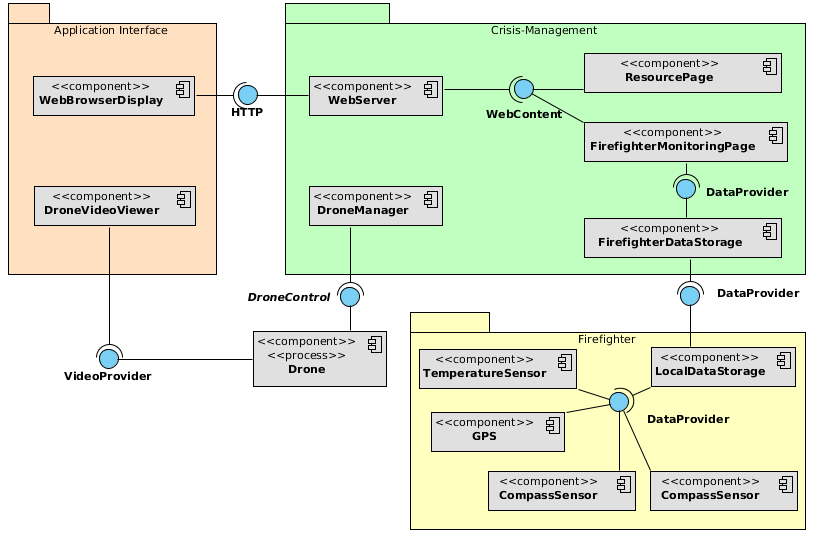
\includegraphics[scale=0.4]{./chapter5/figures/complete-usecase-new2}
	\caption{\label{fig:complete-usecase}The component configuration for our crisis-management use-case.}
\end{figure*}

Every use case we present extends the crisis-management base application by any one of the following possibilities: adding new or redundant components, adding external Java applications with wrapper components (e.g., Weka, DaCapo), or modifying existing components (e.g., to introduce a fault into them).
Using this template in the experiments allow us to measure the behavior of our proposal in a more realistic environment where many components with different features co-exist.
%is extended in every use case by: modifying existent components (e.g, to introduce faulty behavior), adding new redundant components and adding external java applications with a wrapper component.
%The particular features of each component are details in each experiment.

\subsection{Measurement Methodology} \label{sec:measurement_metodology}
To obtain comparable and reproducible results, we used the same hardware across all experiments: a laptop with a 2.90GHz Intel(R) i7-3520M processor, running Fedora 19 with a 64 bit kernel and 8GiB of system memory.
We used the HotSpot Java Virtual Machine version 1.7.0\_67, and Kevoree framework version 5.0.1.
Each measurement presented in the experiment is the average of ten different runs under the same conditions. 
%In addition to the template application we presented, we introduce a new component to execute an external jar file. This new component is used to measure the impact of the faulty behavior on the execution of the system by measuring its execution time.

The evaluation of our approach is tightly coupled with the quality of the resource consumption contracts attached to each component.
We built the contracts following classic profiling techniques. 
The contracts were built by performing several runs of our use cases, without inserting any faulty components into the execution.
Firstly, we executed the use cases in an environment with global monitoring activated to get information for the global contract.
Secondly, per-component contracts were created by running the use cases in an environment with full monitoring.

\subsection{Overhead of the instrumentation solution\label{sec:OverheadFullMonitoring}}
Our first experiment compares the various instrumentation levels to show the overhead of each one. 
In this section, \emph{Memory instrumentation} refers to the technique for accounting memory which leverage bytecode instrumentation, while \textit{Heap Exploration} refers to the memory accouting technique which leverage on-demand heap exploration.
%The results of the evaluation are fundamental because they justify the interest of our adaptative monitoring approach. 
%Additionally, these results are the baseline to understand the rest of the evaluation. 
In this experiment, we compare the following instrumentation levels: \emph{No monitoring}, \emph{Global monitoring}, \emph{Memory instrumentation}, \emph{Instructions instrumentation}, \emph{Memory and instructions instrumentation} (i.e., Full monitoring).
We also evaluate the impact on performance of the two fine-grain memory monitoring approaches we proposed: instrumentation-based and heap-dump-based.

In this set of experiments we used the DaCapo 2006 benchmark suite \cite{Blackburn:2006:DBJ:1167473.1167488}. 
We developed a Kevoree component to execute this benchmark~\footnote{\url{http://goo.gl/V5T6De}}.
The container was configured to use full monitoring and the parameters in the contract are upper bounds of the real consumption\footnote{Scripts are generated from those available at \url{http://goo.gl/FR8LC7}.}.

\begin{figure}[!ht]
\centering
\begin{tikzpicture}
\begin{axis}[
every axis legend/.append style={nodes={right}},
ybar=0pt,
legend style={at={(0.25,1.1)},
anchor=north,legend columns=1, font=\tiny},
ylabel={Time (seconds)},
y label style={at={(0.04, 0.5)}},
scaled y ticks = false,
      y tick label style={/pgf/number format/fixed,
      /pgf/number format/1000 sep = \thinspace % Optional if you want to replace comma as the 1000 separator 
      },
xtick=data,ymin=0,
width = 13cm,
height = 5cm,
bar width = 6,
x tick label style={rotate=45,anchor=east, font=\small},
 axis lines*=left, % Don't display the top and right lines
 symbolic x coords={antlr,fop,hsqldb,jython,chart,luindex,xalan,lusearch}
]
\addplot[fill=black] coordinates 
	{(antlr,1.28) (fop,1.101) (hsqldb,2.337) (jython,2.351) (chart,2.534) (luindex,3.561) (xalan,1.224) (lusearch,1.305)};
\addplot[fill=gray] coordinates 
	{(antlr,1.023) (fop,1.039) (hsqldb,2.284) (jython,2.524) (chart,2.417) (luindex,3.165) (xalan,1.191) (lusearch,1.321)};
\addplot[pattern=north east lines] coordinates 
	{(antlr,2.164) (fop,1.188) (hsqldb,8.655) (jython,10.688) (chart,4.806) (luindex,8.001) (xalan,4.885) (lusearch,9.349)};
\addplot[pattern=crosshatch] coordinates 
	{(antlr,6.235) (fop,1.905) (hsqldb,9.091) (jython,10.905) (chart,8.985) (luindex,44.988) (xalan,8.026) (lusearch,9.261)};
\addplot[pattern=dots] coordinates 
	{(antlr,7.468) (fop,1.970) (hsqldb,15.888) (jython,18.625) (chart,11.502) (luindex,51.660) (xalan,11.188) (lusearch,18.975)};
\legend{No monitoring, Global monitoring, Memory instrumentation,Instructions instrumentation, Memory \& Instructions instrumentation}
\end{axis}
\end{tikzpicture}
\caption{Execution time for tests using the DaCapo Benchmark\label{overhead-of-monitoring}}
\end{figure}

Figure \ref{overhead-of-monitoring} shows the execution time of several DaCapo tests under different scenarios when only instrumentation is used to provide fine-grain monitoring.
First, we wish to highlight that \emph{Global monitoring} introduces no overhead compared with the \emph{No monitoring} mode.
Second, the overhead due to memory accounting is lower than the overhead due to instruction accounting.
This is very important because, as we described in section \ref{monitorContainer}, memory probes cannot be deactivated dynamically.

To perform the comparison, we evaluate the overhead produced for each monitoring mode. We calculated the overhead as: \[overhead=\frac{WithInstrumentation}{GlobalMonitoring}\]

The average overhead due to instruction accounting is 5.62, while the value for memory accounting depends on the monitoring mechanism.
If bytecode instrumentation is used, the average overhead is 3.29 which is close to the values reported in \cite{Binder:2009:PPV:1464245.1464249}.
In the case of instruction accounting, these values are not as good as the values reported in \cite{Binder:2009:PPV:1464245.1464249}; because they obtain a better value between 3.2 and 4.3 for instructions accounting.
The performance difference comes from a specific optimization that we chose not to apply.
The optimization provides fast access to the execution context by adding a new parameter to each method.
Nevertheless, this solution needs to keep a version of the method without the new parameter because native calls cannot be instrumented like that. 
We decided to avoid such an optimization because duplication of methods increases the size of the applications, and with it, the memory used by the heap.
In short, our solution can reach similar values if we include the mentioned optimization, but at the cost of using more memory.
On the other hand, the values we report are far lower than the values reported in \cite{Binder:2009:PPV:1464245.1464249} for hprof.
Hence, we consider that our solution is comparable to state of the art approaches in the literature.

In Figure~\ref{overhead-of-monitoring-with_heapexplorer} we compare the execution time of the same benchmarks but using different memory monitoring approaches.
This comparison is important because, as explained in section~\ref{monitorContainer}, the two approaches have different CPU footprint.
These are controlled experiments where, in order to stress the technique, we demand the execution of a \textit{heap exploration} step every two seconds, which is not the expected usage pattern.
On the contrary, the memory instrumentation technique is executed with the expected usage pattern.
In comparison to using memory instrumentation where the average execution time is 3.29, the average overhead in execution time  decreases to 1.79 if the \textit{Heap Exploration} monitoring mechanism is used.
This value is better than the value reported in \cite{Binder:2009:PPV:1464245.1464249}.
These results suggest that this technique has less impact on the behavior of applications being monitored.

\begin{figure}[!ht]
\centering
\begin{tikzpicture}
\begin{axis}[
every axis legend/.append style={nodes={right}},
ybar=0pt, legend style={at={(0.25,1.1)},
anchor=north,legend columns=1, font=\tiny},
ylabel={Time (seconds)},
y label style={at={(0.04, 0.5)}},
scaled y ticks = false,
      y tick label style={/pgf/number format/fixed,
      /pgf/number format/1000 sep = \thinspace % Optional if you want to replace comma as the 1000 separator 
      },
xtick=data,ymin=0,
width = \textwidth,
height = 5cm,
bar width = 6,
x tick label style={rotate=45,anchor=east, font=\small},
 axis lines*=left, % Don't display the top and right lines
 symbolic x coords={antlr,fop,hsqldb,jython,chart,luindex,xalan,lusearch}
]
% no monitoring
\addplot[fill=black] coordinates 
	{(antlr,1.28) (fop,1.101) (hsqldb,2.337) (jython,2.351) (chart,2.534) (luindex,3.561) (xalan,1.224) (lusearch,1.305)};
% memory
\addplot[pattern=north east lines] coordinates 
	{(antlr,2.164) (fop,1.188) (hsqldb,8.655) (jython,10.688) (chart,4.806) (luindex,8.001) (xalan,4.885) (lusearch,9.349)};
% heap dump
\addplot[pattern=crosshatch dots] coordinates 
	{(antlr,1.143) (fop,1.125) (hsqldb,8.639) (jython,2.762) (chart,2.836) (luindex,3.589) (xalan,1.822) (lusearch,5.078)};
% memory and instructions
\addplot[pattern=dots] coordinates 
	{(antlr,7.468) (fop,1.970) (hsqldb,15.888) (jython,18.625) (chart,11.502) (luindex,51.660) (xalan,11.188) (lusearch,18.975)};
% heap dump and instructions
\addplot[fill=white] coordinates 
	{(antlr,6.159) (fop,1.188) (hsqldb,14.647) (jython,10.950) (chart,9.059) (luindex,44.758) (xalan,7.812) (lusearch,15.990)};
% legend
\legend{No Monitoring, Memory instrumentation, Heap Exploration, Memory \& Instructions instrumentation, Heap Exploration \& Instructions Instrumentation}
\end{axis}
\end{tikzpicture}
\caption{Comparison of execution time for tests using two different memory monitoring techniques\label{overhead-of-monitoring-with_heapexplorer}}
\end{figure}

The results of our experiment shown in Figures~\ref{overhead-of-monitoring} and~\ref{overhead-of-monitoring-with_heapexplorer} demonstrate the extensive impact of the \emph{Full monitoring} mode, which uses either \emph{Memory instrumentation} or \emph{CPU instrumentation}, has on the application. Thus, our \emph{Adaptive monitoring} mode, which uses \emph{Global monitoring} and switches to \emph{Full monitoring} or \emph{localized monitoring}, has the potential to reduce this accumulated overhead due to the fact that \emph{Global monitoring} has no appreciable overhead. 
%The results of the evaluation are fundamentals because they justify the interest of our adaptative monitoring approach. 
%Additionally, these results are the baseline to understand the rest of the evaluation. 

%In addition, we plan to study alternatives to improve instruction accounting. %These alternatives are about using peak monitoring and learning monitoring.
%For example, we plan to study the use of machine learning for monitoring \cite{tesauro2006hybrid}. Based on a machine learning approach, it is possible to train the monitoring system to do the instruction instrumentation. Then, instead of doing normal instruction instrumentation, we might only do, for example, method-calls instrumentation and with the learning data, the monitoring system should be able to infer the CPU usage of each call, whilst lowering the overhead.

\subsection{Overhead of Adaptive Monitoring vs Full Monitoring\label{sec:adaptive-vs-full}}
The previous experiment highlights the potential of using \emph{Adaptive monitoring}. However, switching from \emph{Global monitoring} to either \emph{Full} or \emph{Localized monitoring} introduces an additional overhead due to having to instrument components and activate monitoring probes.
Our second experiment compares the overhead introduced by the adaptive monitoring with the overhead of \emph{Full monitoring} as used in state-of-the-art monitoring approaches. 
%The result of this experiment shows the potential interest of the adaptive monitoring approach.

Table \ref{use-cases-sheet2} shows the tests we built for the experiment.
We developed the tests by extending the template application. Faults were introduced by modifying an existing component to break compliance with its resource consumption contract.
We reproduce each execution repetitively; thus, the faulty behaviour is triggered many times during the execution of the application. The application is not restarted.
%\hl{We selected as heuristic in almost every case \textit{number-of-failures} which is the best because there is only a single faulty component.}\todo{must be explain later}

\begin{table*}[!hb]
\centering
\caption{Features of use cases.\label{use-cases-sheet2}}
\begin{tabular}{|c|p{2.1cm}|p{1.4cm}|p{2cm}|p{2.5cm}|}
\hline Test Name & Monitored\newline Resource & Faulty\newline Resource & Heuristic & External Task \\ 
\hline UC1 & CPU, Memory & CPU & number\newline of failures & Weka, training neural network \\ 
\hline UC2 & CPU, Memory & CPU & number\newline of failures & dacapo, antlr \\ 
\hline UC3 & CPU, Memory & CPU & number\newline of failures & dacapo, chart \\ 
\hline UC4 & CPU & CPU & number\newline of failures & dacapo, xalan \\ 
\hline UC5 & CPU, Memory & CPU & less number\newline of failures\newline first  & dacapo, chart \\ 
\hline UC6 & Memory & CPU & number\newline of failures & Weka, training neural network \\ 
\hline 
\end{tabular} 
\end{table*}


Figure \ref{adaptive-vs-full} shows the execution time of running the use cases with different scenarios.
Each scenario uses a specific monitoring policy (\emph{Full monitoring}, \emph{Adaptive monitoring with All Components}, \emph{Adaptive monitoring with Localized monitoring}, \emph{Global monitoring}).
All these scenarios were executed with the heap explorer memory monitoring policy. 
This Figure shows that the overhead differences between \textit{Full monitoring} and \emph{Adaptive monitoring with All Components} is clearly impacted by scenarios that cause the system to transition too frequently between a lightweight Global and a fine-grain \emph{Adaptive monitoring}.
Such is the case for use cases UC3 and UC4 because the faulty component is inserted and never removed.
%As we explained in section \ref{analysis}, 
Using \emph{Adaptive monitoring} is beneficial if the overhead of \emph{Global monitoring} plus the overhead of switching back and forth to \emph{All Components monitoring} is less than the overhead of the \emph{Full monitoring} for the same execution period.
If the application switches between monitoring modes too often then the benefits of adaptive monitoring are lost.

The overhead of switching from \emph{Global monitoring} to \emph{full components} or \emph{Localized monitoring} comes from the fact that the framework must reload and instrument classes to activate the monitoring probes.
Therefore, using \emph{Localized monitoring} reduces the number of classes that must be reloaded.
This is shown in the third use-case of Figure~\ref{adaptive-vs-full}, which uses a heuristic based on the number of failures.
Because we execute the faulty component many times, the heuristic is able to select, monitor and identify the faulty component quickly. This reduces overhead by 93\%. We use the following equation to calculate overhead:

\[ Gain=100-\frac{OurApproach-GlobalMonitoring}{FullMonitoring-GlobalMonitoring}*100 \]

We also evaluate the execution time for each use case using the instrumentation-based memory monitoring mode.
The average gain in that case is 81.49\% and, as shown in previous section, in average it behaves worse than the \textit{Heap Exploration} mechanism.
However, it is worth noting that the difference between using memory monitoring based on instrumentation and heap exploration is less remarkable than in the previous experiment.
Observe how in test UC4, using a combination of heap exploration and adaptive monitoring with all components behaves worse than using plain instrumentation-based memory monitoring.
In this particular test, activating and deactivating the monitoring probes dominate the execution time.
Alas, adding a heap exploration step right after the probes are activated, just add some extra overhead.
On the contrary, there is no additional step executed when we use instrumentation to measure the memory usage.
Apparently, what matter when the all components strategy is guiding the adaptive monitoring is the ratio among the amount of allocations performed by components and the size of those components.

\begin{figure}
\centering
\begin{tikzpicture}
\begin{axis}[
every axis legend/.append style={nodes={right}},
ybar=0pt, legend style={at={(0.8,1.2)},
anchor=north,legend columns=1, font=\tiny},
ylabel={Time (seconds)},
y label style={at={(0.02, 0.5)}},
scaled y ticks = false,
      y tick label style={/pgf/number format/fixed,
      /pgf/number format/1000 sep = \thinspace % Optional if you want to replace comma as the 1000 separator 
      },
xtick=data,ymin=0,
width = \textwidth,
height = 5cm,
bar width = 6,
x tick label style={rotate=45,anchor=east, font=\small},
 axis lines*=left, % Don't display the top and right lines
 symbolic x coords={UC1,UC2,UC3,UC4,UC5,UC6}
]
% full monitoring
\addplot[fill=black] coordinates 
	{(UC1,613.000) (UC2,46.363) (UC3,63.899) (UC4,78.324) (UC5,49.144) (UC6,132.949)};
% adaptive with all component
\addplot[fill=red, pattern=crosshatch dots] coordinates 
	{(UC1,432.744) (UC2,70.501) (UC3,198.554) (UC4,187.036) (UC5,32.340) (UC6,127.711)};
% adaptive with all component and heap dump
\addplot[fill=yellow, pattern=crosshatch] coordinates 
	{(UC1,410.790) (UC2,61.808) (UC3,95.503) (UC4,204.479) (UC5,16.864) (UC6,123.381)};
% adaptive with heuristic
\addplot[fill=green, pattern=north west lines] coordinates 
	{(UC1,176.413) (UC2,16.741) (UC3,29.461) (UC4,19.470) (UC5,27.001) (UC6,123.813)};
% adaptive with heuristic and heap dump
\addplot[fill=pink, pattern=dots] coordinates 
	{(UC1,169.467) (UC2,12.520) (UC3,16.403) (UC4,20.251) (UC5,15.110) (UC6,124.294)};
% global monitoring
\addplot[fill=cyan, pattern=north east lines] coordinates 
	{(UC1,166.759) (UC2,10.646) (UC3,14.37) (UC4,20.860) (UC5,14.77) (UC6,120.16)};
\legend{
	Full monitoring, 
	Adaptive with All Components using Memory Instrumentation, 
	Adaptive with All Components using Heap Exploration, 
	Localized monitoring using Memory Instrumentation, 
	Localized monitoring using Heap Exploration,
	Global Monitoring}
\end{axis}
\end{tikzpicture}
\caption{Execution time for some use cases under different monitoring policies.}\label{adaptive-vs-full}
\end{figure}

\subsection{Overhead from switching monitoring modes, and the need of a good heuristic\label{sec:switch-heuristic}}
As we explain in the previous experiments, even if using \emph{Localized monitoring} is able to reduce the overhead of the monitoring system, the switch between \emph{Global} and \emph{Localized monitoring} introduces additional overhead.
If this overhead is too high, the benefits of adaptive monitoring are lost.

In this experiment we show the impact of the application's size, in terms of number of components, and the impact of the component's size, in terms of number of classes, on adaptive monitoring. We also show that the choice of the heuristic to select suspected components for monitoring is important to minimize the overhead caused from repeated instrumentation and probe activation processes.

For the use case, we created two components and we introduced them into the template application separately.
Both components perform the same task, which is performing a \textit{primality test} on a random number and sending the number to another component.
However, one of the components causes 115 classes to be loaded, while the other only loads 4 classes.
%An additional component is in charge of generating random numbers to be consumed by the primality tester components.

We used the same basic scenario with a varying number of \textit{primality testing's} components and component sizes.
In this way, we were able to simulate the two dimensions of application size.
The exact settings, leading to 12 experiments, are defined by the composition of the following constraints:
\begin{itemize}
	\item $N_{comp} = \left\lbrace 4, 8, 16, 32, 64, 128 \right\rbrace$  which defines the number of components for the application
	\item $Size_{comp}=\left\lbrace 4, 115 \right\rbrace$ which defines the number of classes for a component
\end{itemize} 

With these use cases, we measured the delay to find the faulty component and the execution-time overhead caused by monitoring.
Figures \ref{fig:delay-time-115} and \ref{fig:delay-time-4} show the delay to detect the faulty component with regards to the size of the application.
In the first Figure, the component size is 115 classes, and in the second Figure, the component size is four classes.
%Figures \ref{fig:execution-time-many-115} and \ref{fig:execution-time-many-4} show the overhead of monitoring based on the execution time of the main task and according to the size of the application. In the first one, the component size is 115 classes and in the second one, the component size is four classes.

\begin{figure*}
 \centering
 % 115 classes
 \begin{minipage}[t]{0.45\linewidth}
 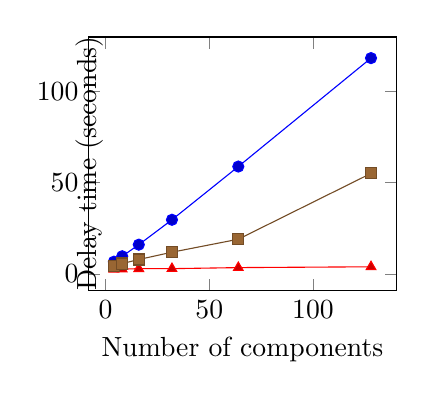
\begin{tikzpicture}
 \begin{axis}[
 	ylabel={Delay time (seconds)},
 	y label style={at={(0.08, 0.5)}},
 	xlabel={Number of components},width = 5.5cm,
 	height = 4.8cm]

 \addplot+[mark=*] coordinates
 	{(4,6.614953125) (8,9.60012962962963) (16,15.9376486486486) (32,29.564) (64,58.7045) (128,118.061571428571)};
 	
 \addplot+[mark=triangle*] coordinates
 	{(4,2.46368292682927) (8,2.56517142857143) (16,2.79086206896552) (32,2.81322222222222) (64,3.3868064516129) (128,3.83251724137931)};
 	
 \addplot+[mark=square*] coordinates
	 	{(4,4.31777777777778) (8,5.59077777777778) (16,7.81511538461538) (32,11.8165)  (64,18.9216363636364) (128,54.9538)};

 \end{axis}
 \end{tikzpicture}
 \caption{Delay time to detect fault with a\newline component size of 115 classes.\label{fig:delay-time-115}}
\end{minipage}
 % 4 classes
 \begin{minipage}[t]{0.45\linewidth}
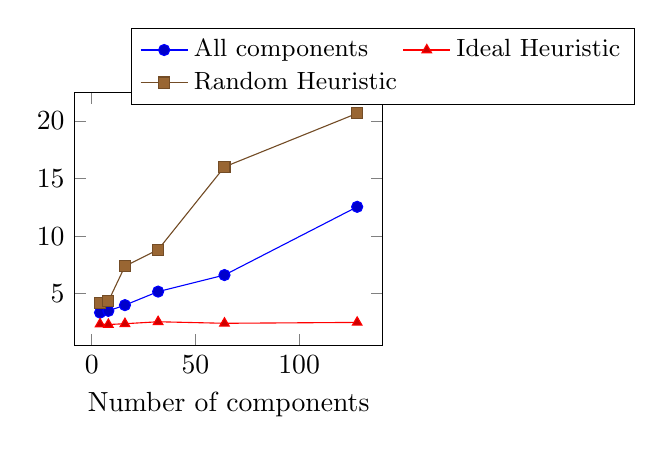
\begin{tikzpicture}
 \begin{axis}[
 	every axis legend/.append style={nodes={right}},
 	legend columns=2, 
 	legend style={at={(1.0,0.95)},
 	anchor=south,legend columns=1, font=\small},
 	xlabel={Number of components},width = 5.5cm,
 	height = 4.8cm]

 \addplot+[mark=*] coordinates
 	{(4,3.36101408450704) (8,3.51326153846154) (16,4.01246031746032) (32,5.18675) (64,6.62437704918033) (128,12.5490980392157)};
 	
 \addplot+[mark=triangle*] coordinates
 	{(4,2.3682619047619) (8,2.32882926829268) (16,2.39802777777778) (32,2.568) (64,2.43528571428571) (128,2.51225806451613)};
 	
 \addplot+[mark=square*] coordinates
	 	{(4,4.18407692307692) (8,4.35309090909091) (16,7.392) (32,8.82909090909091)  (64,16.017125) (128,20.6681428571429)};

	\legend{All components, Ideal Heuristic, Random Heuristic}
 \end{axis}
 \end{tikzpicture}
%\caption{4 classes}
 \caption{Delay time to detect fault with a\newline component size of four classes.\label{fig:delay-time-4}}
 \end{minipage}
\hspace{1cm}
\end{figure*}

 \begin{figure*}
 \centering
 % 115 classes
 \begin{minipage}[t]{0.45\linewidth}
 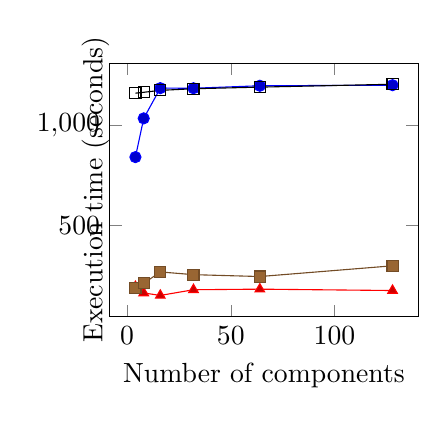
\begin{tikzpicture}
 \begin{axis}[
 	ylabel={Execution time (seconds)},
 	y label style={at={(0.03, 0.5)}},
 	xlabel={Number of components},width = 5.5cm,
 	height = 4.8cm]

 \addplot+[mark=*] coordinates
 	{(4,842.274) (8,1035.734) (16,1186.657) (32,1186.140) (64,1198.539) (128,1201.415)};
 	
 \addplot+[mark=triangle*] coordinates
 	{(4,195.609) (8,163.964) (16,151.637) (32,180.026) (64,182.962) (128,176.101)};
 	
 \addplot+[mark=square*] coordinates
	 	{(4,186.798) (8,211.913) (16,268.908) (32,255.329)  (64,245.976) (128,299.516)};
	 	
 \addplot+[mark=square] coordinates
	 	{(4,1161.593) (8,1165.910) (16,1175.643) (32,1183.620)  (64,1191.749) (128,1206.128)};
 \end{axis}
 \end{tikzpicture}
 \caption{Execution time of main\newline task with a component size\newline of 115 classes.\label{fig:execution-time-many-115}}
\end{minipage}
 % 4 classes
 \begin{minipage}[t]{0.45\linewidth}
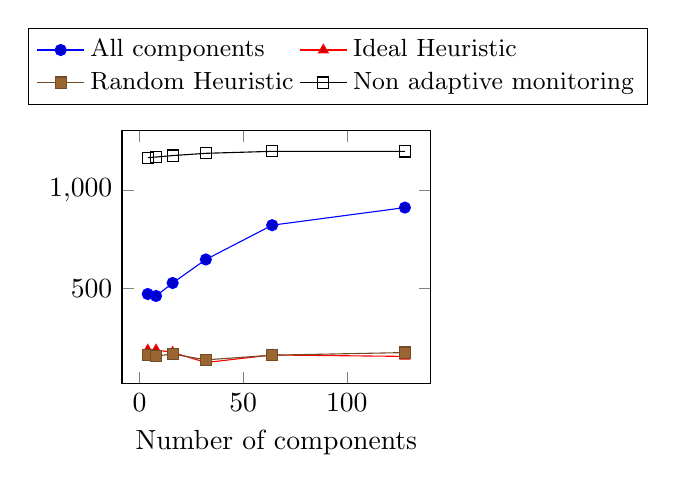
\begin{tikzpicture}
 \begin{axis}[
 	every axis legend/.append style={nodes={right}},
 	legend columns=2,
 	legend style={at={(0.7,1.1)},
 	anchor=south,legend columns=1, font=\small},
 	xlabel={Number of components},width = 5.5cm,
 	height = 4.8cm]

\addplot+[mark=*] coordinates
 	{(4,471.532) (8,461.274) (16,527.667) (32,647.634) (64,822.767) (128,912.634)};
 	
 \addplot+[mark=triangle*] coordinates
 	{(4,185.003) (8,185.533) (16,173.457) (32,121.551) (64,160.201) (128,152.802)};
 	
 \addplot+[mark=square*] coordinates
	 	{(4,161.985) (8,154.983) (16,164.704) (32,135.131)  (64,159.032) (128,172.392)};
	 	
 \addplot+[mark=square] coordinates
	 	{(4,1167.814) (8,1170.811) (16,1178.219) (32,1189.748)  (64,1199.834) (128,1199.453)};

	\legend{All components, Ideal Heuristic, Random Heuristic, Non adaptive monitoring}
 \end{axis}
 \end{tikzpicture}
 \caption{Execution time of main\newline task with a component size\newline of four classes.\label{fig:execution-time-many-4}}
 \end{minipage}
\hspace{1.5cm}
\end{figure*}


\subsubsection{Impact of the application size}
%\paragraph{Impact of the application size}
Figures \ref{fig:delay-time-4} and \ref{fig:execution-time-many-4} show the size of the application has an impact on the delay to detect faulty components, and also on the monitoring overhead.
We also calculated the time needed to find the faulty component with the \emph{All components} mode after its initialization (the time needed to switch from \emph{Global monitoring}).
This time is around 2 seconds no matter the size of the application.
That is the reason the switch from \emph{Global monitoring} to \emph{All components} has such a large effect on overhead.

These figures also show that using \emph{Localized monitoring} instead of \emph{All components} when switching from \emph{Global monitoring} helps reduce the impact of the application's size by reducing the number of components to monitor and the number of classes to instrument.
However, we also see that using a sub-optimal heuristic may have negatively impacted the delay to detect faulty components.
This can be explained by the multiple switches that the Random heuristic may often require to locate the faulty component.

\subsubsection{Impact of the component size}
%and \ref{fig:execution-time-many-115}, \ref{fig:execution-time-many-4}
In Figures \ref{fig:delay-time-115} and \ref{fig:delay-time-4} we can observe that the component size greatly impact the performance and the delay for ScapeGoat to find the faulty component. 
Similar to the explanation for the application's size, component size impacts the switch from \emph{Global monitoring} to \emph{Localized monitoring}, because of the class reloading and instrumentation.
A good heuristic drastically reduces the number of transitions; thus, it has a huge impact on the delay. 
When the components size increase, the choice of a good heuristics becomes even more important, because the cost of dynamic monitoring probes injection increase with the size of the components.
\section{Scapegoat to spot faulty components in a scalable diverse web application}\label{sec:WebStudy}
In this section, we present another application that benefits from the Scapegoat approach.
Although the general goal of spotting components that behave abnormally regarding resource consumption remains the same, with this use case we highlight the possibility of using Scapegoat 
%on a real application 
%and a specific usage of Scapegoat 
to automatically find buggy components on a scalable modular web application.
The section \ref{MdMS} presents an introduction to the application use case, while the remainder of the section deals with the experimental setup and the results.


\subsection{Use case presentation}\label{MdMS}
We are applying the Scapegoat approach to check resource consumption contracts on a web application called MdMS.\footnote{\url{https://github.com/maxleiko/mdms-ringojs}}
This application offers a web Content Management System based on the Markdown language for editing posts. 
MdMS uses a typical architecture (as shown in Figure \ref{fig:webapp}) for scalable web applications: a load-balancer connected to a set of workers (called MdMS Sosie in Figure \ref{fig:webapp}), which are themselves connected to a distributed database to retrieve the application specific content.
The worker layer of this application can be duplicated across various machines to support a growing number of clients.
The web application is currently online\footnote{\url{http://cloud.diversify-project.eu/}}. 

\begin{figure*}[!bt]
	\centering
	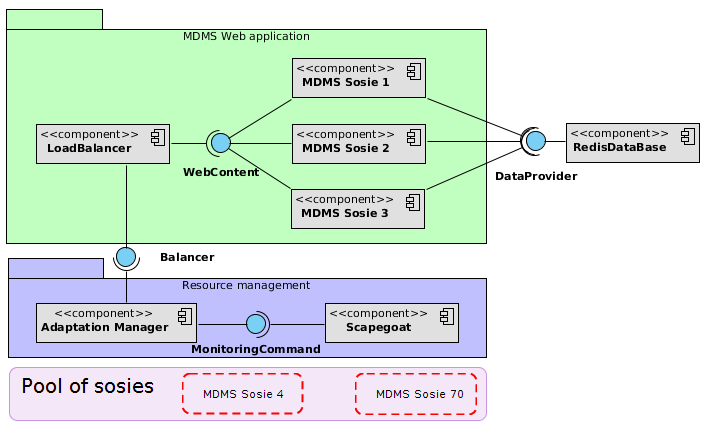
\includegraphics[scale=0.45]{./chapter5/figures/webapp2}
	\caption{\label{fig:webapp}Architecture of MdMS along with Scapegoat and additional components to adapt the system.}
\end{figure*}

The main characteristic of MdMS is that workers are not pure clones but diverse implementations of the MdMS server stack~\cite{alliermulti}.
This proactive diversification of MdMS targets safety~\cite{avizienis85} and security~\cite{Forrest97} purposes.
In particular, we have used a recent technique for the automatic synthesis of \textit{sosie} programs~\cite{baudry2014tailored} in order to automatically diversify the workers. 
A \textit{sosie} is a variant of a program that exhibits the same functionality (passes the same test suite) and a diverse computation (different control or data flow). 
\textit{Sosie} synthesis is based on the transformation of the original program through statement deletion, addition or replacement.
%The MdMS application is leveraging this diversified set of workers in order to reach the scalability property while icluding diversity in the software layer to prevent the so-called BOBE (Blow Once, Blow Everywhere) attacks~\cite{alliermulti}.

While the construction of \textit{sosies} focuses on preserving functional correctness, it ignores all the non-functional aspects of the program.
Consequently, a \textit{sosie} offers no guarantee regarding its resource consumption and may contain memory leaks or other overhead on resource consumption that can significantly impact the performance of MdMS.

In this experiment, we use Scapegoat to monitor the resource consumption of the various \textit{sosies} of the MdMS workers.
This technique enables us to identify \textit{sosies} in a production environment that do not behave according to the resource consumption contracts, allowing the system to remove these workers and use other \textit{sosies}.
Our goal in this experiment is to answer the following question:

\begin{itemize}
 \item Does Scapegoat correctly identify the faulty components in a system which includes many variants of the same component?   
\end{itemize}

\subsection{Experimental setup}

We devised this experiment as a scenario where many clients interact with the web application at the same time by adding and removing articles.
The stress produced by these requests increases the resource consumption on the server side which is running on top of Kevoree components.
Figure~\ref{fig:webapp} depicts the server side's configuration.
Since MdMS is a web application developed on top of RingoJS~\footnote{\url{https://github.com/ringo/ringojs}}, a JavaScript runtime written in Java, our \textit{sosies} include the RingoJS framework and the application that has been wrapped into Kevoree components.

In this experiment, we deploy many of these components as back-end servers of the web application and we use Scapegoat to monitor the consumption of each server.
Their contracts regarding resource consumption were built using the mechanism described in section \ref{sec:measurement_metodology} but with the original MdMS worker as a reference component.
The application also contains a component acting as a front-end that evenly distributes the requests among back-end servers.
This load balancer implements a plain round robin policy.
%There is an additional component running on the platform, it is in charge of adapting the system.
%This component reacts to events produced by Scapegoat and modifies the deployed system following the Models@run.time paradigm.

To produce a realistic load on the web server we have recorded a set of standard activities on the MdMS web site using Selenium~\footnote{\url{http://www.seleniumhq.org/}}.
We then use the Selenium facilities to replay these activities many times in parallel to provide the required work load on the server.
% of resource consumption, we generate many accesses to the system.
%We use Selenium~\footnote{http://www.seleniumhq.org/} to accomplish this purpose since MdMS is a web application.
Our experimental settings feature 120 clients which are scheduled by a pool of 7 concurrent Selenium workers.
Each client adds 10 articles to the database through the Website GUI, which represents 16 requests per article, for a total of 19200 requests to the MdMS workers sent through the load balancer.
In this experiment, the Selenium workers are executed on the same physical device as the web server, with the same testing platform described in section~\ref{sec:measurement_metodology}.

The experiment is configured as follows.
Using the diversification technique described in~\cite{baudry2014tailored}, we synthesized 20 \textit{sosies} of the MdMS workers.
These \textit{sosies} are used to execute the application with a varying number of back-ends (from 4 to 10).
One particular \textit{sosie} has been modified by hand to ensure that it violates the original component's contract.
We execute all the described components as well as the Scapegoat components on a single instance of Kevoree.

\subsection{Experimentation results}

Figure~\ref{fig:execution-time-web-app} shows the time required on the server side to reply to all the requests sent by Selenium.
Although the values might look surprisingly high at first, they are in fact the result of a heavily loaded system.
Selenium is actually rendering a couple of web pages for each added article; hence at least 2400 pages are rendered.
Moreover, both clients and servers are sharing resources because they run on the same physical device.
%Another point to highlight is that the time needed to execute all these requests remains stable when no monitoring is used and only changes abruptly when deploying ten \textit{sosies}.
%The execution times remain stable when monitoring is not activated, which is expected because the number of requests does not change between experiments, the load balancer distributes these requests evenly, and we are using the same physical device to execute all back-end servers.
%The stability of the executions when monitoring is not activated is expected because the number of requests does not change between experiments, the load balancer distributes these requests evenly, and we are using the same physical device to execute all back-end servers.
This leads to very stable execution times when monitoring is not activated because the number of requests does not change between experiments, the load balancer distributes these requests evenly, and we are using the same physical device to execute all back-end servers.
%\todo{Please, read below the explanation for: Why the execution time decreases?}
In the \textit{local monitoring} series, the global time to execute decreases until reaching 9 \textit{sosies}.
Although counterintuitive, it is caused by the effect of having \textit{localized monitoring} and \textit{load balancing} at the same time.
For instance, when four \textit{sosies} are used, the monitoring probes are periodically injected into one component out of four, hence roughly a quarter of the requests are handled by a slower \textit{sosie}.
However, with eight components the slow execution path is only taken by around 12.5\% of the requests.
The overhead of \textit{Localized monitoring} when ten \textit{sosies} are deployed increases because the physical machine reaches its limit and begins thrashing.
As a consequence, low-level interactions with the hardware (e.g. cache misses), the operating system and the JVM slow down the execution.
On average, the overhead due to monitoring with both instruction instrumentation and memory instrumentation is 1.59, which is lower than the values shown in section~\ref{sec:OverheadFullMonitoring} for full monitoring despite only one of the instrumentation mechanisms being enabled in those experiments.
The values in this section are better even if we are monitoring both resources because we are using the adaptive approach.
   

\begin{figure*}
 \centering
 \begin{minipage}[t]{0.43\linewidth}
 \centering
 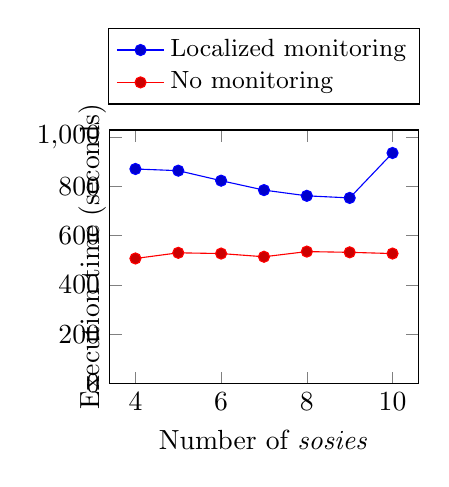
\begin{tikzpicture}
  \begin{axis}[
  	ylabel={Execution time (seconds)},
  	y label style={at={(0.02, 0.5)}},
  	legend style={at={(0.5,1.1)},
  	 	 	anchor=south,legend columns=1, font=\small},
  	ymin=0,
  	every axis legend/.append style={nodes={right}},
  	xlabel={Number of \textit{sosies}},width = 5.5cm,
  	height = 4.8cm]
 
  \addplot+[mark=*] coordinates
  	{(4, 870.375) (5, 863.5) (6, 822.875) (7, 784.625) (8, 761.375) (9, 752.875) (10, 935.3)};

\addplot+[mark=*] coordinates
  	{(4, 507) (5, 530) (6, 527) (7, 514) (8, 535) (9, 532) (10, 527)};
  	
  	\legend{Localized monitoring, No monitoring}
  	
  \end{axis}
  \end{tikzpicture}
  \caption{Time to obtain the reply to all requests.\label{fig:execution-time-web-app}}
  \end{minipage}
  \hspace{0.1\linewidth}
 \begin{minipage}[t]{0.43\linewidth}
 \centering
 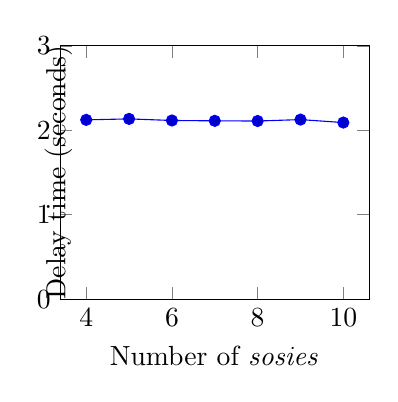
\begin{tikzpicture}
 \begin{axis}[
 	ylabel={Delay time (seconds)},
 	y label style={at={(0.07, 0.5)}}, 	
 	ymin=0,ymax=3,
 	xlabel={Number of \textit{sosies}},width = 5.5cm,
 	height = 4.8cm]

 \addplot+[mark=*] coordinates
 	{(4,2.1235) (5, 2.1348) (6,2.11605) (7,2.1119) (8, 2.1097) (9, 2.12654) (10, 2.09139)};
 	
 \end{axis}
 \end{tikzpicture}
 \caption{Average delay time to detect a faulty \textit{sosie}.\label{fig:delay-time-web-app}}
\end{minipage}

\hspace{1cm}
\end{figure*}


In these experiments, we evaluate the accuracy of the output and its quality in terms of the time needed to find the faulty component.
Scapegoat always spots the correct \textit{sosie}.
It does so because it is an iterative process that continues until finding the faulty component.
In addition, Scapegoat does not output false positives during these experiments.
The delay to detect faulty components is shown in Figure~\ref{fig:delay-time-web-app}.
In this case, the values remain close to 2 seconds no matter the number of \textit{sosies} used nor the execution time.
This behavior is consistent with the experiments in section~\ref{sec:evaluation} because we are also using a good heuristic for the use case.
It shows that Scapegoat can spot faulty components with an acceptable delay in a real application.

\subsection{Discussion of the use case}
This use case shows that Scapegoat is able to provide useful information in real applications.
It also highlights how the framework can help select software variants at runtime in the context of software diversity.
Or, more generally, in the field of software oriented architectures where many stakeholders may provide the same services, Scapegoat can help to choose services.
Moreover, this use case leads to a distributed usage of Scapegoat, where the policies for admission control and resource consumption monitoring can be coordinated among distributed devices.

Finally, in systems where there are many variants of the same component or service, Scapegoat provides essential information to drive application reconfiguration.
For example, the adaptation component in Figure~\ref{fig:webapp} may use Scapegoat's faulty component selection to replace a faulty \textit{sosie} or to modify the scheduling policy in the load balancer.






\section{Threats to validity}
Our experiments show the benefits of using adaptive monitoring instead of state-of-the-art monitoring approaches.
As in every experimental protocol, our evaluation has some bias which we have tried to mitigate.
The experiments are based on a few cases of study. 
We have tried to mitigate this issue by using available real cases study; we have also used different settings across our experiments.
Thus, our experiments limit the validity of the approach to applications with the same characteristics of the presented case study.
New experiments with other use cases are needed to broaden the validation scope of our approach.

The evaluation of the heuristic mainly shows the potential impact of using an ideal heuristic. 
More cases of study and experiments are needed to fully validate the value of our Models@run.time based heuristic.